\documentclass[a4paper]{article}
\setlength{\topmargin}{-1.0in}
\setlength{\oddsidemargin}{-0.2in}
\setlength{\evensidemargin}{0in}
\setlength{\textheight}{10.5in}
\setlength{\textwidth}{6.5in}
\usepackage{enumitem}
\usepackage{amsmath}
\usepackage{hyperref}
\usepackage{amssymb}
\usepackage[dvipsnames] {xcolor}
\usepackage{mathpartir}
\usepackage{graphicx}
\usepackage{tikz}
\usetikzlibrary{positioning,arrows.meta}

\hbadness=10000

\hypersetup{
    colorlinks=true,
    linkcolor=blue,
    filecolor=magenta,      
    urlcolor=cyan,
    pdftitle={Assignment 2},
    pdfpagemode=FullScreen,
    }
\def\endproofmark{$\Box$}
\newenvironment{proof}{\par{\bf Proof}:}{\endproofmark\smallskip}
\begin{document}
\begin{center}
{\large \bf \color{red}  Department of Computer Science} \\
{\large \bf \color{red}  Ashoka University} \\

\vspace{0.1in}

{\large \bf \color{blue}  Introdution to Quantitative Finance}

\vspace{0.05in}

    { \bf \color{YellowOrange} Assignment 2}
\end{center}
\medskip

\hfill {\textbf{Name: Rushil Gupta} }

\bigskip
\hrule


% Begin your assignment here %

\section*{Question 1}
We can solve this problem by linear programming. We can define the variables as follows:

\begin{align*}
    x &= \text{Number of Super Dark bars} \\
    y &= \text{Number of Special Dark bars}
\end{align*}

The objective is to maximize the profit, which is given by:

\begin{align*}
    P = 1x + 2y
\end{align*}

The constraints are:

\begin{align*}
    90x + 80y &\leq 1260 \\
    10x + 20y &\leq 240 \\
    x &\geq 0 \\
    y &\geq 0
\end{align*}

By solving this, we find that the chocolatier should create 0 bars of Super Dark and 12 bars of Special Dark. $(x = 0, y = 12)$

\vspace{10mm}
\section*{Question 2}
We have the following variables:

\begin{align*}
    x_i &= \text{Binary variable indicating if project } i \text{ is selected (1 if selected, 0 otherwise)}
\end{align*}

The objective is to maximize the total returns:

\begin{align*}
    \text{Maximize } \sum_{i=1}^{5} r_i x_i \quad \quad \text{(where } \quad r_i \text{ is the return for project } i \text{)}
\end{align*}

The constraints are:

\begin{align*}
    \sum_{i=1}^{5} e_{j,i} x_i &\leq 25 \quad \forall {j \in \{1, 2, 3\}} \quad \text{(where } e_{j,i} \text{ is the expenditure for project } i \text{ in Year } j)
\end{align*}

Using the PuLP solver, we find that the projects that should be selected are Projects 1, 2, 3, and 4. This allows us to earn a maximum profit of Rs. 95 Cr.


\newpage
\section*{Question 3}

We first need to make a decision tree, where each node represents a state (the number of fish in the lake at the start of the season) and each edge represents a decision (to fish or not), and the value of the edge is the profit for that decision. We can then use the decision tree to find the optimal strategy. In this method, we also use discounting, since when we add the NPV of the future profits, we multiply the profit of that decision by a discount factor, in this case $\frac{1}{1.33}$.

\begin{center}
\begin{tikzpicture}[
    node distance=0.5cm and 2cm,
    node_style/.style={draw=black, fill=white, circle, minimum size=40pt, inner sep=0pt, align=center},
    edge_style/.style={font=\small}
]

% Root node
\node[node_style] (S1) {10 tons};

% Level 1
\node[right=of S1,yshift=1cm,node_style] (S2A) {20 tons};
\node[right=of S1,yshift=-1.5cm,node_style] (S2B) {10 tons};

% Edges from Season 1 to Season 2
\draw[edge_style] (S1) edge node[fill=white,inner sep=2pt] {0} (S2A);
\draw[edge_style] (S1) edge node[fill=white,inner sep=2pt] {7} (S2B);

% Level 2
\node[right=of S2A,yshift=1cm,node_style] (S3A) {40 tons};
\node[right=of S2A,yshift=-1.5cm,node_style] (S3B) {20 tons};
\node[right=of S2B,yshift=-1.5cm,node_style] (S3C) {10 tons};

% Edges from Season 2A
\draw[edge_style] (S2A) edge node[fill=white,inner sep=2pt] {0} (S3A);
\draw[edge_style] (S2A) edge node[fill=white,inner sep=2pt] {14} (S3B);

% Edges from Season 2B
\draw[edge_style] (S2B) edge node[fill=white,inner sep=2pt] {0} (S3B);
\draw[edge_style] (S2B) edge node[fill=white,inner sep=2pt] {7} (S3C);

% Level 3
\node[right=of S3A, yshift=1cm,node_style] (S4A) {80 tons};
\node[right=of S3A, yshift=-1.5cm,node_style] (S4B) {40 tons};
\node[right=of S3B, yshift=-1.5cm,node_style] (S4C) {20 tons};
\node[right=of S3C, yshift=-1.5cm,node_style] (S4D) {10 tons};

% Edges from Season 3A
\draw[edge_style] (S3A) edge node[fill=white,inner sep=2pt] {0} (S4A);
\draw[edge_style] (S3A) edge node[fill=white,inner sep=2pt] {28} (S4B);

% Edges from Season 3B
\draw[edge_style] (S3B) edge node[fill=white,inner sep=2pt] {0} (S4B);
\draw[edge_style] (S3B) edge node[fill=white,inner sep=2pt] {14} (S4C);

% Edges from Season 3C
\draw[edge_style] (S3C) edge node[fill=white,inner sep=2pt] {0} (S4C);
\draw[edge_style] (S3C) edge node[fill=white,inner sep=2pt] {7} (S4D);

\end{tikzpicture}
\end{center}

Now, we can use dynamic programming to find the optimal strategy. We can start at the end of the tree and work our way back to the start. While doing this, at each node, we will store the highest NPV possible from that node to the end of the tree.

\begin{center}
    \begin{tikzpicture}[
        node distance=0.5cm and 2cm,
        node_style/.style={draw=black, fill=white, circle, minimum size=35pt, inner sep=0pt, align=center},
        edge_style/.style={font=\small}
    ]
    
    % Root node
    \node[node_style, ultra thick] (S1) {18.44};
    
    % Level 1
    \node[right=of S1,yshift=1cm,node_style, ultra thick] (S2A) {24.53};
    \node[right=of S1,yshift=-1.5cm,node_style] (S2B) {12.26};
    
    % Edges from Season 1 to Season 2
    \draw[edge_style, ultra thick] (S1) edge node[fill=white,inner sep=2pt] {0} (S2A);
    \draw[edge_style] (S1) edge node[fill=white,inner sep=2pt] {7} (S2B);
    
    % Level 2
    \node[right=of S2A,yshift=1cm,node_style] (S3A) {28};
    \node[right=of S2A,yshift=-1.5cm,node_style, ultra thick] (S3B) {14};
    \node[right=of S2B,yshift=-1.5cm,node_style] (S3C) {7};
    
    % Edges from Season 2A
    \draw[edge_style] (S2A) edge node[fill=white,inner sep=2pt] {0} (S3A);
    \draw[edge_style, ultra thick] (S2A) edge node[fill=white,inner sep=2pt] {14} (S3B);
    
    % Edges from Season 2B
    \draw[edge_style] (S2B) edge node[fill=white,inner sep=2pt] {0} (S3B);
    \draw[edge_style] (S2B) edge node[fill=white,inner sep=2pt] {7} (S3C);
    
    % Level 3
    \node[right=of S3A, yshift=1cm,node_style] (S4A) {0};
    \node[right=of S3A, yshift=-1.5cm,node_style] (S4B) {0};
    \node[right=of S3B, yshift=-1.5cm,node_style, ultra thick] (S4C) {0};
    \node[right=of S3C, yshift=-1.5cm,node_style] (S4D) {0};
    
    % Edges from Season 3A
    \draw[edge_style] (S3A) edge node[fill=white,inner sep=2pt] {0} (S4A);
    \draw[edge_style] (S3A) edge node[fill=white,inner sep=2pt] {28} (S4B);
    
    % Edges from Season 3B
    \draw[edge_style] (S3B) edge node[fill=white,inner sep=2pt] {0} (S4B);
    \draw[edge_style, ultra thick] (S3B) edge node[fill=white,inner sep=2pt] {14} (S4C);
    
    % Edges from Season 3C
    \draw[edge_style] (S3C) edge node[fill=white,inner sep=2pt] {0} (S4C);
    \draw[edge_style] (S3C) edge node[fill=white,inner sep=2pt] {7} (S4D);
    
\end{tikzpicture}
\end{center}


\newpage

\section*{Question 4}

We know that the 2 bullets are loaded consecutively, and in the current situation, we have already shot an empty round. The first round being empty means that the first bullet was not in the first or the last slot. This means that we must be in one of the 4 slots initially. \\

The probability that the next round is a bullet is then the probability that the first bullet is in one of the even slots, which is $\frac{1}{4}$. \\

If we decide to spin the barrel before shooting, the probability of the bullet being in the next chamber is $\frac{2}{6}$ = $\frac{1}{3}$. \\

Hence, spinning the barrel before shooting is worse, as it lowers the probability of the bullet being in the next chamber.


\vspace{10mm}

\section*{Question 5}

\begin{enumerate}[label=(\alph*)]
    \item To determine c, we need to ensure that the integral of the joint PDF over the entire range equals 1.

    \begin{align*}
        \int_{0}^{2} \int_{1}^{3} c(x^2 + xy + y^2) \, dy \, dx = 1
    \end{align*}

    We can solve this by first integrating with respect to y:

    \begin{align*}
        \int_{0}^{2} \left[ c \left( x^2 y + \frac{xy^2}{2} + \frac{y^3}{3} \right) \right]_{1}^{3} \, dx = 1
    \end{align*}

    Solving the integral, we get:
    \begin{align*}
        \int_{0}^{2} c \left( x^2(3 - 1) + \frac{x(3^2 - 1^2)}{2} + \frac{3^3 - 1^3}{3} \right) \, dx = \int_{0}^{2} c \left( 2x^2 + 4x + \frac{26}{3} \right) \, dx = 1
    \end{align*}

    Now, integrating with respect to x, we get:
    \begin{align*}
        c \left( \frac{2x^3}{3} + 2x^2 + \frac{26x}{3} \right) \bigg|_{0}^{2} = 1
    \end{align*}

    Solving this, we get:
    \begin{align*}
        c \left( \frac{16}{3} + 8 + \frac{52}{3} \right) = 1 \implies c \left( \frac{16 + 24 + 52}{3} \right) = 1 \implies c \left( \frac{92}{3} \right) = 1 \implies c = \frac{3}{92}
    \end{align*}

    \vspace{5mm}
    \item \begin{align*}
        E[X] &= \int_{0}^{2} \int_{1}^{3} x \cdot c(x^2 + xy + y^2) \, dy \, dx \\
        &= \int_{0}^{2} \int_{1}^{3} x \cdot \frac{3}{92} (x^2 + xy + y^2) \, dy \, dx \\
        &=  \frac{3}{92} \int_{0}^{2} \left( 2x^3 + 4x^2 + \frac{26x}{3} \right) dx \\
        &=  \frac{3}{92} \left( \frac{2x^4}{4} + \frac{4x^3}{3} + \frac{26x^2}{6} \right) \bigg|_{0}^{2} \\
        &=  \frac{3}{92} \left( 8 + \frac{32}{3} + \frac{26 \cdot 4}{6} \right) \\
        &= 1.174
    \end{align*}

    \begin{align*}
        E[Y] &= \int_{0}^{2} \int_{1}^{3} y \cdot c(x^2 + xy + y^2) \, dy \, dx \\
        &= \frac{3}{92} \int_{0}^{2} \int_{1}^{3} \left( x^2y + xy^2 + y^3 \right) \, dy \, dx \\
        &= \frac{3}{92} \int_{0}^{2} \left( \frac{x^2 y^2}{2} + \frac{xy^3}{3} + \frac{y^4}{4} \right) \bigg|_{1}^{3} \, dx \\
        &= \frac{3}{92} \int_{0}^{2} \left( 4x^2 + \frac{26x}{3} + 20 \right) \, dx \\
        &= \frac{3}{92} \left( \frac{4x^3}{3} + \frac{26x^2}{6} + 20x \right) \bigg|_{0}^{2} \\
        &= \frac{3}{92} \left( \frac{32}{3} + \frac{52}{3} + 40 \right) \\
        &= 2.217
    \end{align*}

    \begin{align*}
        E[XY] &= \int_{0}^{2} \int_{1}^{3} xy \cdot c(x^2 + xy + y^2) \, dy \, dx \\
        &= \frac{3}{92} \int_{0}^{2} x \int_{1}^{3} \left( x^2y + xy^2 + y^3 \right) \, dy \, dx \\
        &= \frac{3}{92} \int_{0}^{2} \left(4x^3  + \frac{26x^2}{3} + 20x \right) \, dx \\
        &= \frac{3}{92} \left( x^4 + \frac{26x^3}{9} + 10x^2 \right) \bigg|_{0}^{2} \\
        &= \frac{3}{92} \left( 16 + \frac{26 \cdot 8}{9} + 40 \right) \\
        &= 2.580
    \end{align*}

    \vspace{5mm}
    \item For $X$ and $Y$ to be statistically independent, $E[XY] = E[X]E[Y]$. We can see that this is not the case here, since $E[XY] = 2.58 \neq 2.603 = 1.174 \times 2.217 = E[X]E[Y]$.
    
    \vspace{5mm}
    \item We first begin by calculating the probability distribution of $X$ given $Y = y_0$. We can do this by using the formula for conditional probability:

    \begin{align*}
        g(x) &= \frac{f_{X,Y}(x, y_0)}{f_Y(y_0)}
    \end{align*}

    Note that in this case, $y_0 = E[Y] = 2.217$.

    \begin{align*}
        f_Y(y_0) &= \frac{3}{92} \int_{0}^{2} (x^2 + xy_0 + y_0^2) \, dx \\
        &= \frac{3}{92} \left( \frac{8}{3} + 2y_0 + 2y_0^2 \right) \\
        &= \frac{3}{92} \left( \frac{8}{3} + 2 \cdot 2.217 + 2 \cdot (2.217)^2 \right) \\
        &= \frac{3}{92} \left( \frac{8}{3} + 4.434 + 10.23 \right) \\
        &= \frac{3}{92} \cdot 17.997 \\
        &= 0.552
    \end{align*}

    \begin{align*}
        f_{X,Y}(x, y_0) &= c(x^2 + xy_0 + y_0^2) \\
        &= \frac{3}{92} (x^2 + 2.217x + (2.217)^2)
    \end{align*}
    \begin{align*}
        g(x) &= \frac{f_{X,Y}(x, y_0)}{f_Y(y_0)} \\
        &= \frac{3}{92} \cdot \frac{x^2 + 2.217x + 4.915}{0.552}
    \end{align*}

    Now, to find $E[X|Y = y_0]$, we can simply evaluate the following integral:

    \begin{align*}
        E[X|Y = y_0] &= \int_{0}^{2} x \cdot g(x) \, dx \\
        &= \int_{0}^{2} x \cdot \frac{3}{92} \cdot \frac{x^2 + 2.217x + 4.915}{0.552} \, dx = 1.166
    \end{align*}

    To find the variance of $X$ given $Y = y_0$, we can use the following formula:

    \begin{align*}
        Var(X|Y = y_0) &= E[X^2|Y = y_0] - (E[X|Y = y_0])^2 \\
        E[X^2|Y = y_0] &= \int_{0}^{2} x^2 \cdot g(x) \, dx \\
        &= \int_{0}^{2} x^2 \cdot \frac{3}{92} \cdot \frac{x^2 + 2.217x + 4.915}{0.552} \, dx = 1.676
    \end{align*}

    Therefore, $Var(X|Y = y_0) = 1.676 - (1.166)^2 = 0.3164$
\end{enumerate}

\vspace{5mm}

\section*{Question 6}

\begin{enumerate}[label=(\alph*)]
    \item $\text{Mean return = }0.0022$, $\text{Risk} = 0.0999$

    \item $\text{Within } \sigma = 68.33\%, \quad \text{Within } 2\sigma = 95.36\%, \quad \text{Within } 3\sigma = 99.74\%$

    \item Histogram of returns:
    \begin{figure}[h]
        \centering
        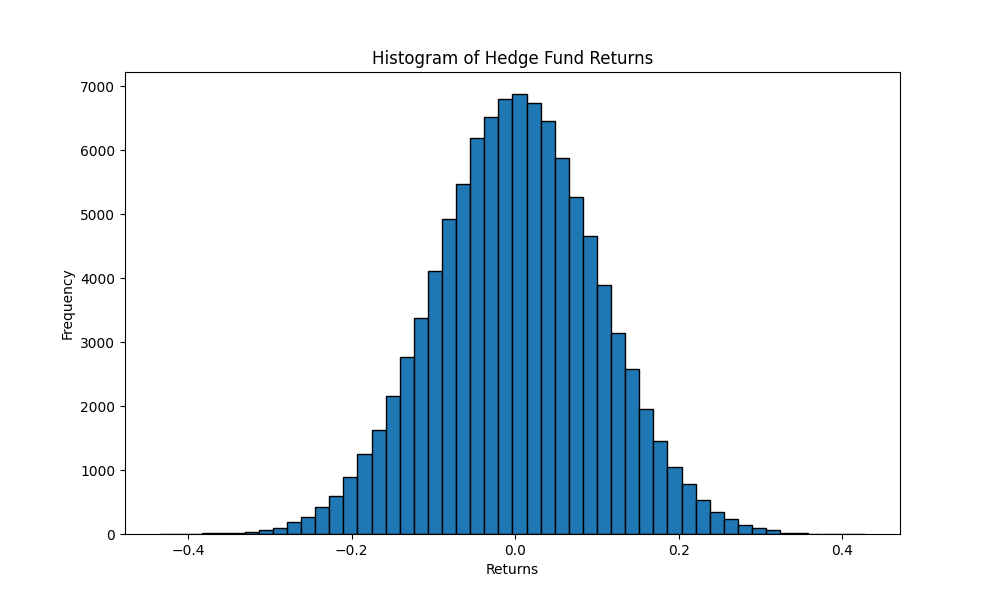
\includegraphics[width=0.8\textwidth]{q6.png}
    \end{figure}
\end{enumerate}

\newpage
\section*{Question 7}

% You can invest in only two risky assets, A and B. Asset A has an expected return of 20 percent with a standard deviation (risk) of 50 percent, while Asset B offers an expected return of 15 percent with a standard deviation of 33 percent. The two assets are uncorrelated with each other.

% \begin{enumerate}[label=(\alph*)]
%     \item Calculate portfolio expected return and portfolio risk (standard deviation) if an investor invests 10 percent in A and the remaining 90 percent in B.

%     \item Generalize the above calculations for portfolio return and risk by assuming an investment of $w_A$ in Asset A and an investment of $(1 - w_A)$ in Asset B. Plot the investment opportunity set for all the values of $w_A$.

%     \item Now introduce a risk-free asset with a return of 3 percent. Write an equation for the capital allocation line in terms of $w_A$ that will connect the risk-free asset to the portfolio of risky assets (you are investing $w_A$ in Asset A and $(1 - w_A)$ in risk free asset).

%     \item Calculate the equation of the capital allocation line with the maximum slope. Also, calculate the investment distribution between Asset A and the risk-free asset corresponding to the maximum slope.

%     \item For capital allocation line determined in part (d), what is the risk of portfolios with returns of 3 percent, 9 percent, 15 percent, and 20 percent on the capital allocation line (i.e., portfolios constructed using Asset A and the risk-free asset in different proportions)? If your risk aversion coefficient A0 is 2.5, what is the utility you derive from each of these portfolios?
% \end{enumerate}

% Hint: $U = E(r) - \frac{1}{2} A \sigma^2$ \\

% Where:
% \begin{itemize}
%     \item U is Utility: Represents the investor's satisfaction from holding a portfolio.
%     \item E(r) is Expected Return: The average return on the portfolio.
%     \item A is Risk Aversion Coefficient: Measures how much risk the investor is willing to take. Higher A means more risk-averse.
%     \item $\sigma^2$ is Variance of Returns: Reflects the risk or volatility of the portfolio. Higher variance means more uncertainty in returns.
% \end{itemize}
% \end{document}

\begin{enumerate}[label=(\alph*)]
    \item $E(r_p) = 0.1 \cdot 0.2 + 0.9 \cdot 0.15 = 0.155$ \\

    $\sigma_p = \sqrt{0.1^2 \cdot 0.5^2 + 0.9^2 \cdot 0.33^2} = 0.3012 \quad \text{(Since correlation coefficient = 0)}$

    \vspace{5mm}
    \item $E(r_{w_A}) = w_A \cdot 0.2 + (1 - w_A) \cdot 0.15$ \\
    $\sigma_{w_A} = \sqrt{w_A^2 \cdot 0.5^2 + (1 - w_A)^2 \cdot 0.33^2}$ \\

    The plot below shows the portfolio expected return and standard deviation for all values of $w_A \in [0, 1]$.
    \begin{figure}[h]
        \centering
        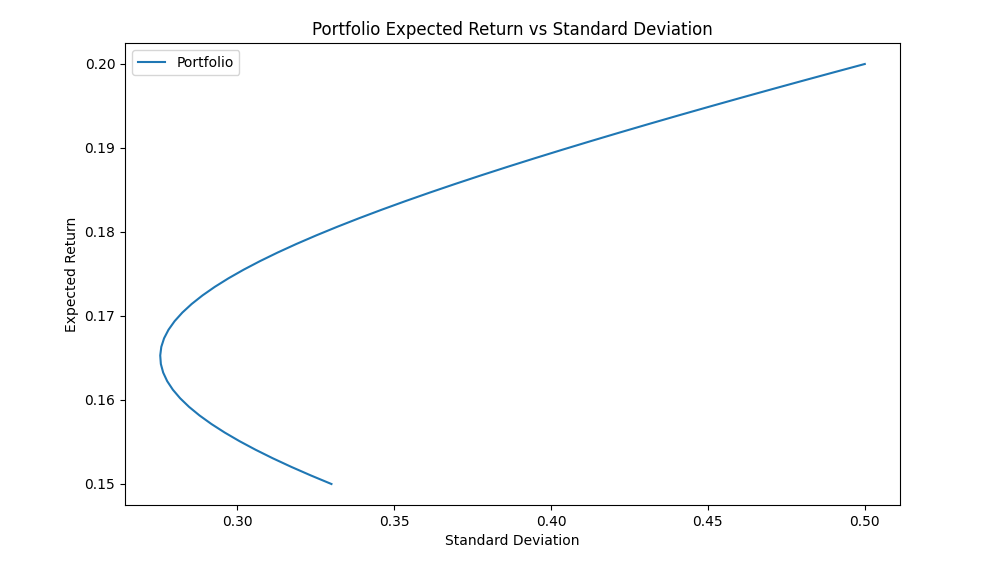
\includegraphics[width=0.8\textwidth]{q7.png}
    \end{figure}

    \vspace{5mm}
    \item The calculate the equation of this line, we need to first find it's slope:
    \[
        m = \frac{0.20 - 0.03}{0.50} = 0.34 \quad \text{(A straight line since no-correlation)}
    \]
    \[
        \implies r_p = 0.34 \sigma_p + 0.03
    \]

    To find this in terms of $w_A$, we can use the following steps:
    \[
        \sigma_p = \sqrt{w_A^2 \cdot 0.5^2 + (1 - w_A)^2 \cdot 0^2} = 0.5w_A
    \]
    \[
        \implies r_p = 0.34 \cdot 0.5w_A + 0.03 = 0.17w_A + 0.03
    \]

    \vspace{5mm}
    \item To find the portfolio with the maximum slope, we need to find the portfolio with the highest expected return for a given level of risk. This is given by the formula:
    \[
        \frac{E(r_{w_A}) - r_f}{\sigma_{w_A}} = \frac{w_A \cdot 0.2 + (1 - w_A) \cdot 0.15 - 0.03}{\sqrt{w_A^2 \cdot 0.5^2 + (1 - w_A)^2 \cdot 0.33^2}}
    \]

    By taking the derivative and setting it to 0, we can find the value of $w_A$ that maximizes the slope, which is $w_A = 0.3816 = 38.16\%$. The corresponding maximum slope is $0.4978$.

    \vspace{5mm}
    \item The table below shows the risk, return, and utility for different portfolios on the capital allocation line with the maximum slope. We use the same equations as part b, but set asset A as (0.2794, 0.1691) (the portfolio with the maximum slope) and asset B as (0, 0.03) (the risk free asset).
    
    \begin{table}[h]
        \centering
        \begin{tabular}{|c|c|c|}
            \hline
            Return & Risk & Utility \\
            \hline
            0.03 & 0.0 & 0.0300 \\
            \hline
            0.09 & 0.1205 & 0.0718 \\
            \hline
            0.15 & 0.2410 & 0.0774 \\
            \hline
            0.20 & 0.3415 & 0.0543 \\
            \hline
        \end{tabular}
    \end{table}

\end{enumerate}


\newpage

\section*{Question 8}

\begin{enumerate}[label=(\alph*)]
    \item Point A is not achievable as it is on the left/above the efficient frontier. This is easy to show, since if Point A was achievable, it would dominate some points on the efficient frontier. However, since the efficient frontier dominates all other points, Point A cannot be achievable. \\
    
    \item Points C and G will not be chosen by a rational, risk-averse investor, as it has the same risk as other points on the efficient frontier, but lower returns. This is equivalent to saying that Points C and G are on the right of the efficient frontier, and hence are dominated by other points on the efficient frontier. \\
    
    \item A risk neutral investor is one who is only concerned with the expected return of a portfolio. Since Point D has the highest expected return, it is the most suitable for a risk-neutral investor. \\

    \item Gold is on the inefficient part of the feasible set. Nonetheless, gold is owned by many rational investors as part of a larger portfolio. This is because of 2 major reasons: 1) gold is a safe asset, and hence, it is held by risk averse investors as a diversifier. Moreover, since gold is said to be negatively correlated with stocks, it helps to reduce the overall risk. 2) Gold lies on the inefficient part of the feasible set for this model, but not every investor agrees with the model. This is because the model has 2 major assumptions: i) Every investor is a mean-variance investor, and ii) Each investor has the same information and agree on the same probability distribution. In reality, not every investor agrees with these assumptions, and hence, they may choose to invest in assets that lie on the inefficient part of the feasible set. \\

    \item The utility of an investor at point P with a risk aversion coefficient of 3 is:
    \[
        U = E(r) - \frac{1}{2} A \sigma^2 = 0.16 - \frac{1}{2} \cdot 3 \cdot 0.17^2 = 0.16 - 0.04335 = 0.11665
    \]
\end{enumerate}

\end{document}